\documentclass[a4paper]{article}
\usepackage[spanish]{babel}
\usepackage[utf8]{inputenc}
\usepackage{fancyhdr}
\usepackage{charter}   % tipografia
\usepackage{graphicx}
\usepackage{makeidx}

\usepackage{float}
\usepackage{amsmath, amsthm, amssymb}
\usepackage{amsfonts}
\usepackage{sectsty}
\usepackage{wrapfig}
\usepackage{listings}
\usepackage{caption}

\usepackage{hyperref} %las entradas del índice tienen links
\hypersetup{
    colorlinks=true,
    linktoc=all,
    citecolor=black,
    filecolor=black,
    linkcolor=black,
    urlcolor=black
}

\usepackage{color} % para snipets de codigo coloreados
\usepackage{fancybox}  % para el sbox de los snipets de codigo

\definecolor{litegrey}{gray}{0.94}

% \newenvironment{sidebar}{%
% 	\begin{Sbox}\begin{minipage}{.85\textwidth}}%
% 	{\end{minipage}\end{Sbox}%
% 		\begin{center}\setlength{\fboxsep}{6pt}%
% 		\shadowbox{\TheSbox}\end{center}}
% \newenvironment{warning}{%
% 	\begin{Sbox}\begin{minipage}{.85\textwidth}\sffamily\lite\small\RaggedRight}%
% 	{\end{minipage}\end{Sbox}%
% 		\begin{center}\setlength{\fboxsep}{6pt}%
% 		\colorbox{litegrey}{\TheSbox}\end{center}}

\newenvironment{codesnippet}{%
	\begin{Sbox}\begin{minipage}{\textwidth}\sffamily\small}%
	{\end{minipage}\end{Sbox}%
		\begin{center}%
		\colorbox{litegrey}{\TheSbox}\end{center}}



\usepackage{fancyhdr}
\pagestyle{fancy}

%\renewcommand{\chaptermark}[1]{\markboth{#1}{}}
\renewcommand{\sectionmark}[1]{\markright{\thesection\ - #1}}

\fancyhf{}

\fancyhead[LO]{Sección \rightmark} % \thesection\
\fancyfoot[LO]{\small{Martín Caravario, Federico Hosen, Lucas Vuotto}}
\fancyfoot[RO]{\thepage}
\renewcommand{\headrulewidth}{0.5pt}
\renewcommand{\footrulewidth}{0.5pt}
\setlength{\hoffset}{-0.8in}
\setlength{\textwidth}{16cm}
%\setlength{\hoffset}{-1.1cm}
%\setlength{\textwidth}{16cm}
\setlength{\headsep}{0.5cm}
\setlength{\textheight}{25cm}
\setlength{\voffset}{-0.7in}
\setlength{\headwidth}{\textwidth}
\setlength{\headheight}{13.1pt}

\renewcommand{\baselinestretch}{1.1}  % line spacing


\usepackage{underscore}
\usepackage{caratula}
\usepackage{url}

\usepackage{color}
\usepackage{clrscode3e} % para el pseudocodigo




\begin{document}

\lstset{
  language=C++,
  backgroundcolor=\color{white},   % choose the background color
  basicstyle=\footnotesize,        % size of fonts used for the code
  breaklines=true,                 % automatic line breaking only at whitespace
  captionpos=b,                    % sets the caption-position to bottom
  commentstyle=\color{mygreen},    % comment style
  escapeinside={\%*}{*)},          % if you want to add LaTeX within your code
  keywordstyle=\color{blue},       % keyword style
  stringstyle=\color{mymauve},     % string literal style
}

\thispagestyle{empty}
\materia{Sistemas Operativos}
\submateria{Segundo Cuatrimestre de 2014}
\titulo{Trabajo Práctico I}
%\subtitulo{}
\integrante{Caravario, Martín}{470/12}{martin.caravario@gmail.com}
\integrante{Hosen, Federico}{825/12}{fhosen@hotmail.com}
\integrante{Vuotto, Lucas}{385/12}{lvuotto@dc.uba.ar}

\maketitle
\newpage

\thispagestyle{empty}
\vfill
\thispagestyle{empty}
\vspace{1.5cm}
\tableofcontents
\newpage


%\normalsize
\newpage

\section{Introducción}
En este trabajo práctico se realizarán implementaciones de diversos
schedulers, y se analizará su comportamiento de acuerdo a distintas
métricas. Este analisis será realizado con un simulador proporcionado por la
cátedra, el cual describe los procesos del scheduler en cada uno de los
núcleos del procesador, en funcion del tiempo.

\subsection{Métricas utilizadas}
Para realizar este trabajo se debieron utilizar diversas métricas con el
objetivo de analizar distintos aspectos del rendimiento y comportamiento de
los schedulers implementados.

Como las distintas métricas nos pueden arrojar diversas conclusiones sobre
qué scheduler es mejor que otro, se procederá a realizar un análisis
riguroso de cada algoritmo de scheduling bajo las diferentes métricas, con
el fin de obtener una mejor comparación y poder ver las ventajas y
desvantajas de cada algoritmo en distintos ámbitos, como ser el tiempo total
de carga del CPU o la cantidad de procesos finalizados respecto al tiempo
total de uso del CPU.

En este trabajo usaremos se decidieron analizar 3 aspectos:

\begin{itemize}
  \item \textbf{Fairness}: esta métrica, tambien llamada de ecuanimidad,
  captura que tan uniforme es la distribucion del cpu para cada proceso.
  Esto significa que medirá la cantidad de ciclos de CPU que utiliza cada
  proceso, y que tan justa es esa distribución con respecto a los demas. En
  nuestro caso consideramos una distribución justa, que cada proceso tenga
  la misma
  unidad de tiempo.
  \item \textbf{Turnaround}: esta métrica muestra el tiempo total que le
  toma a cada proceso en ejecutar completamente, incluídos los tiempos de
  carga y cambios de contexto.
  \item \textbf{Waiting Time}: ésta métrica nos indica cuanto tiempo pasa
  una tarea esperando a ser ejecutada.
\end{itemize}

Existen otras métricas como por ejemplo el \textit{tiempo de respuesta}, que
se encarga de medir el tiempo de respuesta percibido por el usuario,
que no fueron consideradas a la hora de testear los schedulers ya que
no contabamos con las herramientas necesarias para medir esto. Tampoco
tuvimos en cuenta la medida de \textit{latencia}, la cual mide el tiempo que
necesita un proceso para empezar a dar resultados, debido a que no
conocíamos que hacía cada proceso y no podíamos observar dichos resultados.
\newpage


\section{Ejercicio 1}

\subsection{Explicación del algoritmo}
Para este ejercicio se decidió crear una función llamada \textbf{get\_rand}
a la cual se le pasan los parámetros \textit{bmin} y \textit{bmax}. El
objetivo de esta función es generar un número aleatorio entre \textit{bmin}
y \textit{bmax}, lo cual se lleva de la siguiente manera:

\begin{verbatim}
return rand() % (bmax - bmin + 1) + bmin;
\end{verbatim}

Cabe destacar que utilizamos la funcion \verb|rand|, la cual fue sugerida
por la cátedra, con el fin de generar un numero aleatorio. Esta función es
invocada $n$ veces, siendo $n$ la cantidad de llamados bloqueantes que debe
realizar la tarea, con el fin de generar los números aleatorios que serán
utilizados como la duración de cada llamada.

\section{Ejercicio 2}
En este ejercicio se simulara el scheduler \textit{FCFS} con 3 tareas, una 
intensiva en CPU y las otras dos de tipo TaskConsola. A continuación se
muestra el lote utilizado:
\begin{verbatim}

TaskCPU 12
TaskConsola 0 9 72
TaskConsola 6 1 16

\end{verbatim}

\subsection{Resultados}

\begin{figure}[htb]
\begin{center}
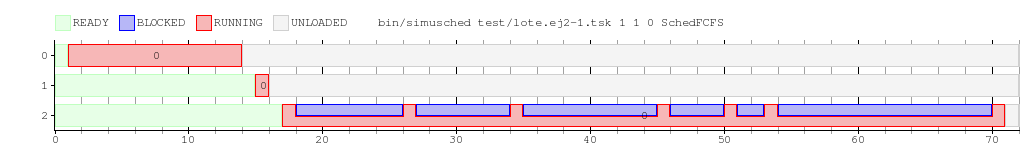
\includegraphics[scale=0.4]{imagenes/ej2-1-c-1.png}
\end{center}
\caption{Gráfico de los procesos corriendo en un núcleo}
\end{figure}

\begin{figure}[htb]
\begin{center}
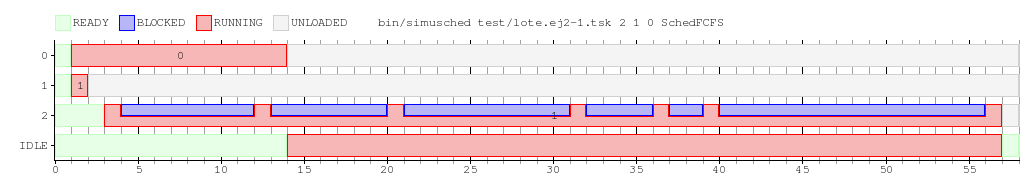
\includegraphics[scale=0.4]{imagenes/ej2-1-c-2.png}
\end{center}
\caption{Gráfico de los procesos corriendo en dos núcleos}
\end{figure}

\begin{figure}[htb]
\begin{center}
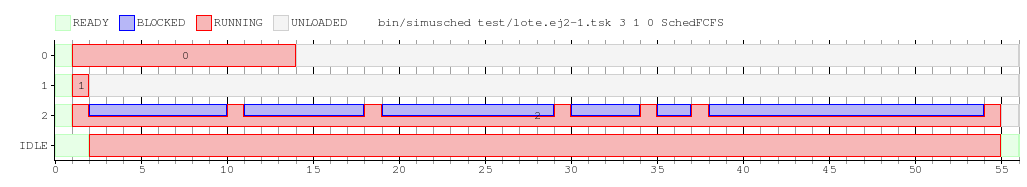
\includegraphics[scale=0.4]{imagenes/ej2-1-c-3.png}
\end{center}
\caption{Gráfico de los procesos corriendo en tres núcleos}
\end{figure}

\newpage

\section{Ejercicio 3: Round Robin}

\subsection{Explicación del algoritmo.}
El tipo de scheduling \textit{round robin} consiste en asignar a cada
proceso un tiempo predeterminado para que se ejecute, llamado
\textit{quantum}. Si el proceso no termina su ejecución antes dicho quantum
se acabe, es desalojado y puesto en una cola (espera circular) para ser
retomada su ejecución luego de atender a los demás procesos en dicha cola.

Este modelo de scheduling permite asegurarse de que no exista la inanición,
pues todos los procesos son atendidos; mas aún, a todos lo
procesos les es asignado el mismo quantum. De esta
forma, round robin es altamente confiable en términos de ecuanimidad.

Para implementarlo utilizamos:
\begin{itemize}
\item una cola \footnote{Implementada con \textit{queue} de la STL de C++.}, de nombre
\textit{ready} que nos indica las tareas en espera para su ejecución.
\item Un vector \footnote{Implementado con
\textit{vector} de la STL de C++.} de enteros \textit{ticks} en el cual
guardamos la cantidad de ciclos restantes para la tarea que está corriendo
en cada núcleo.
\item Un vector de enteros \textit{quantums} donde tenemos
almacenados los quantums correspondientes a cada núcleo. 
\end{itemize}

Dado un núcleo, cuando el elemento de \textit{ticks} correspondiente a dicho
núcleo alcanza el valor $0$, dicho proceso es desalojado y puesto en el
final de la cola, dejando el procesador libre para el próximo en la cola.
Si no existe algún proceso en la cola, el núcleo entra en estado
\textit{idle} hasta que se cargue una nueva tarea.

De igual forma, cuando un proceso se bloquea, es puesto de vuelta en la
cola, y la próxima vez que corra lo hará con el \textit{quantum} entero.
Ésto es, quizás, una de las falencias de esta implementación \textit{naive}
de \textit{round robin} en términos de \textit{fairness}, pues la tarea que
se bloquea \textit{pierde} una porción de su tiempo asignado, que no es
recuperado en su siguiente turno. Una posible modificación a la
implementación para solucionar esto sería añadir algún sistema de
recompensas para las tareas que no terminan su \textit{quantum}.

\section{Ejercicio 4: Simulaciones y análisis de Round Robin}

\subsection{Introducción}
En este ejercicio se analizó el comportamiento del modelo de scheduling
\textit{Round Robin} variando la cantidad de tareas, el quantum, la cantidad
de núcleos y el tiempo de cambio de contexto. Se busca ver cómo estas
variaciones afectan las distintas métricas mencionadas anteriormente, para
así poder arrojar conclusiones sobre este scheduler.

\subsection{Experimento 1: Funcionamiento RR}
En este primer experimento simulamos 8 tareas corriendo simultaneamente en
un procesador de un solo núcleo, fijando el costo de cambio de contexto en 1
y el quantum en 5 ciclos de \textit{clock}. El tiempo en el que cada tarea
pasaba a estado \textit{ready} fue elegido pseudoaleatoriamente.

El objetivo de este experimento fue verificar que la implementación se
comporte en efecto como un scheduler round robin, es decir, que siga el
comportamiento mencionado en el ejercicio 3.

El lote de tareas utilizado fue el siguiente:

\begin{verbatim}
TaskCPU 15
TaskCPU 11
TaskCPU 25
TaskCPU 24
TaskCPU 10
TaskCPU 16
TaskCPU 13
TaskCPU 22
\end{verbatim}


\subsubsection{Resultados}
\begin{figure}[htb]
\begin{center}
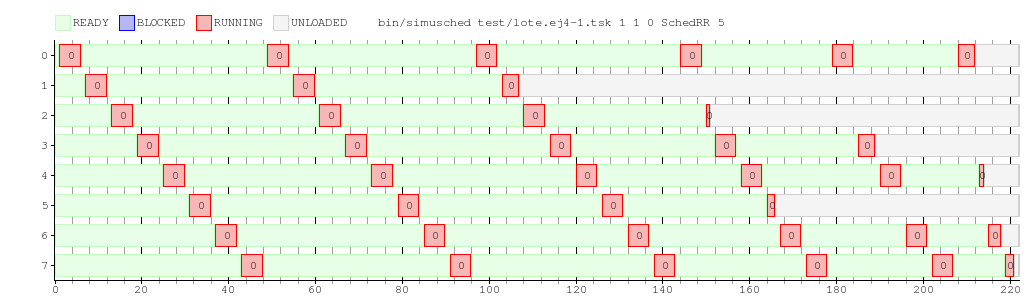
\includegraphics[scale=0.4]{imagenes/ej4-1.png}
\end{center}
\caption{Experimento 1. Lote 8 tareas. Quantum 5.}
\end{figure}

\subsubsection{Conclusión}

Como era de esperarse, empieza a ejecutarse el primer proceso \textit{listo}
hasta cumplir su cuota de tiempo, luego pasa a ejecutar al siguiente, y así
hasta retomar la primer tarea (pues se turnan de manera circular). A medida
que los procesos terminan la totalidad de su ejecución, la cola se va
haciendo más corta, acortando el tiempo de espera entre el desalojo de un
proceso y su retorno. Ésto se repite hasta que todos los procesos terminan
su ejecución.

\section{Ejercicio 5: Lottery Scheduling}
\subsection{Explicación del algoritmo}
El modelo de scheduling \textit{Lottery} consiste en tener un sistema
pseudoaleatorio que decida cual va a ser el siguiente proceso a ser
ejecutado. Esto lo hace \textit{repartiendo tickets} a cada proceso, y
generando un ticket ganador al azar. Así, cada
proceso va a tener asociado una cantidad de tickets, obteniendo
cierta probabilidad de ganar la lotería. De esta forma, el proceso con más
tickets tiene más probabilidades de ganar. Éste es el mecanismo que nos
permite establecer relaciones de prioridades entre procesos.
Y como dado un número entre $1$ y $n$, la posibilidad de que dicho número
\textbf{no} salga nunca es $0$, eventualmente el número será elegido por el
algoritmo de scheduling. De esta forma, no hay \textit{inanición}, pues
todo proceso será puesto a correr en algún momento.

Para implementarlo utilizamos:
\begin{itemize}
\item Una lista de procesos y sus tickets, \textbf{procesos}
\footnote{Utilizamos list(pair(int,int)) de la STL de C++.}.
\item Un diccionario de procesos bloqueados, \textbf{bloqueados}
\footnote{Utilizamos map(int,int) de la STL de C++.}, que dado un pid guarda con cuantos
tickets tiene que regresar.
\item Una variable entera \textbf{ciclos}, que especifica cuantos ciclos
consumió el proceso actual (el que ocupa el procesador).
\item Una variable entera \textbf{quantum}.
\item Una variable entera \textbf{tickets}, que indica la cantidad de
tickets totales asignados.
\end{itemize}

La implementación hecha está basada en la mencionada en el paper. Se utiliza
una lista enlazada para guardar los procesos y sus respectivos tickets.
Inicialmente a todos los procesos se les asigna 1 ticket, teniendo todos las
mismas posibilidades de \textit{salir sorteados}; es interesante notar que
dicho número podría ser cualquiera, mientras sea el mismo para todos, ya que
mantiene la relación de igual prioridad para todos los procesos.

A medida que algunos procesos cambian al estado \textit{bloqueado}, la
cantidad de tickets de éste aumenta en proporción a la fracción de quantum que usó. Al
bloquearse, es agregado al diccionario \textit{bloqueados}, con su pid y
su nueva cantidad de tickets. Luego, al ser desbloqueado, es puesto de nuevo
en la lista con su nueva cantidad de tickets, que es estrictamente mayor a
la cantidad anterior.

Para saber qué proceso debe correr, el scheduler genera un número
aleatorio entre $0$ y $n-1$ \footnote{Siendo $n$ la suma total de tickets}, y luego recorre linealmente la lista de
procesos. Al ir recorriendola, acumula la cantidad de tickets de los
elementos que visita, y cuando dicha suma alcanza el valor generado
ganador se encuentra al ganador.

Una optimización adoptada del paper fue mantener la lista ordenada
decrecientemente, de forma tal que al sacar el número ganador y recorrer la
lista acumulando la sumatoria hasta alcanzar a dicho número, se minimize el
recorrido. Ésto se debe a que los primeros valores son los más grandes,
entonces el valor acumulado aumenta de la forma más rapida posible,
corriendo menos iteraciones para alcanzar dicho valor. Aunque en el peor
caso, el ticket ganador es el $n-1$, con lo cual no importa cómo esté
ordenada la lista, para encontrar al ganador, la lista deberá ser recorrida
hasta el final.

La transferencia de tickets propuesta por el paper no fue implementada, ya que
los procesos simulados en este trabajo no interactúan con otros, con lo cual
no tiene sentido transferir prioridades para mejorar la dependencia entre
procesos. Por la misma razón, tampoco fue implementada la inflación de
tickets, ya que cumple una función similar.

El modelo de \textit{tickets currencies} tampoco fue utilizado, ya que
éste apunta al manejo de recursos compartidos por un grupo de procesos,
situación que no se presenta en estas simulaciones.

\section{Ejercicio 6}

\subsection{Explicación del algoritmo}
Para llevar a cabo el algoritmo se precalculó aleatoriamente en que ciclos
de \textit{clock} el proceso debe bloquearse. Para esto reutilizamos la
función \verb|get_rand| utilizada en el ejercicio 1, con el objetivo de
generar un número pseudoaleatorio entre 0 y la cantidad de ciclos de CPU que
consumirá el proceso. Este número fue utilizado para saber en qué ciclo el
proceso debe bloquearse. Para esto se generó un vector de booleanos (del
tamaño de la cantidad de ciclos que corre la tarea) el cual se llenó en las
posiciones devueltas por la función \verb|get_rand|.

Luego de esto el algoritmo recorre el vector de booleanos y se fija si en
el ciclo actual debe bloquearse o utilizar CPU, según lo que diga esa
posición indexada del vector. 

Cada tarea se bloqueará por un ciclo de \textit{clock}, asegurando así que
el tiempo total utilizado por la tarea es de \textit{total\_cpu} ciclos,
tal como lo pide el enunciado.


\section{Ejercicio 7}

En este experimento analizaremos el impacto del tamaño del quantum en
el tiempo necesario para terminar de ejecutar cada tarea
(\textit{Turnaround}). Asignar un quantum
muy bajo haría que dicho tiempo aumente, dado que habría más ciclos de
\textit{clock} dedicados a realizar los cambios de contextos, aumentando el
tiempo total que le toma a cada tarea terminar su ejecución. Pero si éste es demasiado alto podría generar
que el tiempo de respuesta percibido sea muy alto, pero como no nos interesa
medir esta métrica en estos experimentos, no nos explayaremos más sobre ésto.

Lo que haremos es ir variando el valor del quantum en un procesador de 1
núcleo, y luego variar (con los mismos valores) dicho parámetro en un
procesador de 4 núcleos. Utilizamos el siguiente lote de tareas:

\begin{verbatim}
TaskBatch 10 0 
TaskBatch 10 1
TaskBatch 10 2
TaskBatch 10 3
TaskBatch 10 4
TaskBatch 10 5
TaskBatch 10 6
TaskBatch 10 7
TaskBatch 10 8
\end{verbatim}


Para el propósito del experimento, como nos interesa que las tareas elijan
de forma aleatoria cuando se bloquean y cuando usan CPU, pero al mismo
tiempo nos interesa que esto se mantenga cuando variamos el quantum, y luego
la cantidad de cores, usamos la semilla por defecto ($1$).

Para correr los experimento usamos, como lo pide el enunciado, un costo de
cambio de contexto de $1$, y un costo de migración de $2$.
Estos son los resultados de las simulaciones:

\begin{figure}[H]
\begin{center}
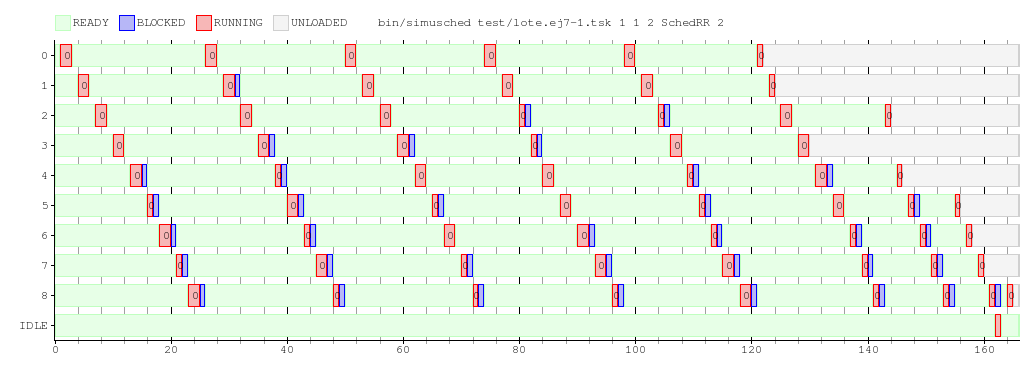
\includegraphics[scale=0.4]{imagenes/ej7-1-c-1-q-2.png}
\end{center}
\caption{Procesador de 1 núcleo, con un quantum de valor 2.}
\end{figure}

\begin{figure}[H]
\begin{center}
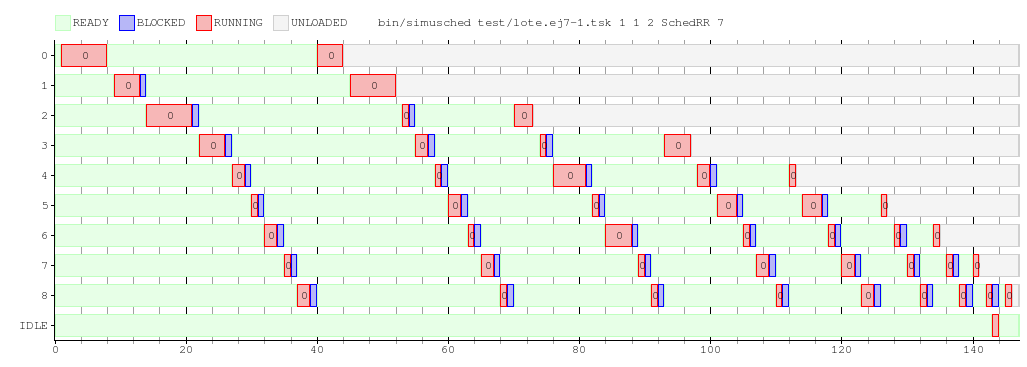
\includegraphics[scale=0.4]{imagenes/ej7-1-c-1-q-7.png}
\end{center}
\caption{Procesador de 1 núcleo, con un quantum de valor 7.}
\end{figure}

\begin{figure}[H]
\begin{center}
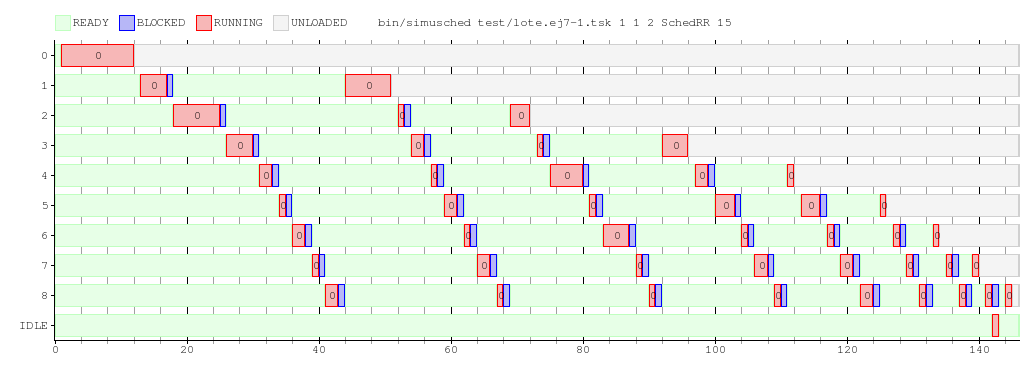
\includegraphics[scale=0.4]{imagenes/ej7-1-c-1-q-15.png}
\end{center}
\caption{Procesador de 1 núcleo, con un quantum de valor 15.}
\end{figure}

\begin{figure}[H]
\begin{center}
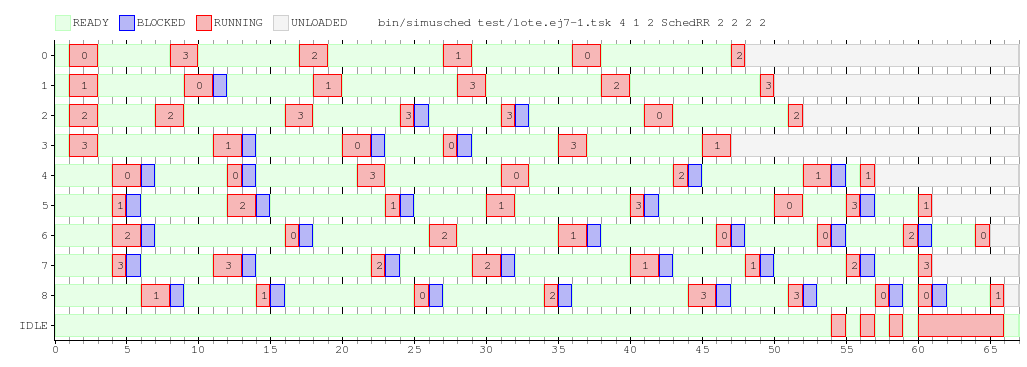
\includegraphics[scale=0.4]{imagenes/ej7-1-c-4-q-2.png}
\end{center}
\caption{Procesador de 4 núcleos, con un quantum de valor 2.}
\end{figure}

\begin{figure}[H]
\begin{center}
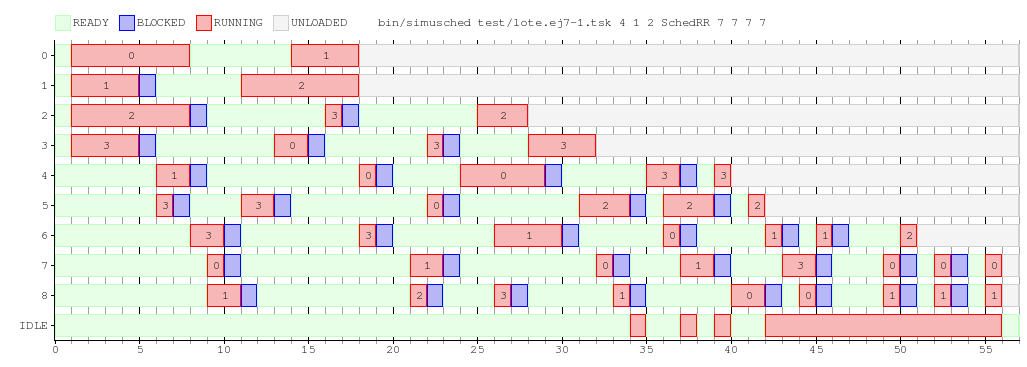
\includegraphics[scale=0.4]{imagenes/ej7-1-c-4-q-7.png}
\end{center}
\caption{Procesador de 4 núcleos, con un quantum de valor 7.}

\end{figure}

\begin{figure}[H]
\begin{center}
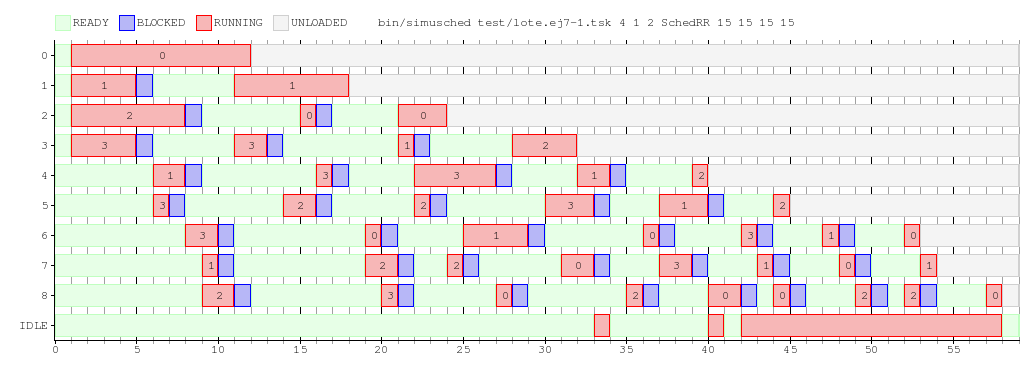
\includegraphics[scale=0.4]{imagenes/ej7-1-c-4-q-15.png}
\end{center}
\caption{Procesador de 4 núcleos, con un quantum de valor 15.}
\end{figure}

\newpage
\subsection{Conclusión}

Si se observa la Figura 2, la tarea $0$ tiene un \textit{turnaround} de 120
(aprox), y el de las demás tareas va aumentando progresivamente (ésto debido
a que el número de llamadas bloqueantes de las tareas aumenta conforme a su
número de tarea).

Por otro lado, en la Figura 3 se observa como el \textit{turnaround} de la
tarea $0$ es de 42, que es significativamente menor a 120. Y progresivamente
el tiempo total de ejecución de las demás tareas va decrementando con respecto
al gráfico anterior.

Entonces, vemos como, a medida que aumenta el quantum se amortiza el costo
de cambio de contexto, pues al durar más el tiempo asignado a cada tarea,
hay menos tiempo \textit{muerto}, tiempo aprovechable para las tareas.

Siguiendo en esta línea, al aumentar el quantum a 15 (figura 4), incluso se observa
como la tarea $0$ puede aprovechar un tiempo asignado tan amplio,
mientras que otras corren de igual forma que en la figura 3.

Los resultados con 4 núcleos no hacen más que reforzar lo analizado
anteriormente. Sucede el mismo fenómeno, con la diferencia de que al tener más
nucleos la totalidad de las tareas terminan antes. La diferencia en términos
de \textit{turnaround} entre un quantum de valor $2$ y otro de valor $7$ es
muy grande, basta con observar a las tareas $0$ a $5$ para notar la mejoría en
el desempeño. Una diferencia interesante con el procesador de $1$ núcleo es
que de un quantum de valor $7$ a uno de valor $15$ sigue habiendo una
mejoría sustancial; ya que, no sólo la tarea $0$ termina antes (como en el
procesador de $1$ núcleo) si no que, también lo hacen las tareas $0$ a $3$.

Podemos concluir entonces, dos puntos. Primero, a medida que el quantum
aumenta, se aprovecha más tiempo del procesador, minimizando los tiempos
muertos generados por los cambios de contexto y migraciones a otros núcleos
, disminuyendo el tiempo total que tarda una tarea en terminar.
Con lo cual, podemos afirmar que al aumentar el quantum nunca va a empeorar 
el desempeño considerando la métrica \textit{turnaround}, al contrario,
va a mejorar, aunque a lo sumo se mantendrá.

Por otro lado, es interesante observar que la mejoría en dicha métrica en
función de incrementar el quantum, está acotada por lo que la tarea hace de
hecho. Ésto es, si la tarea realiza llamadas bloqueantes, no podrá
aprovechar en su totalidad un quantum alto. Dicha situación es observable al
ver la Figura 3 y 4, notar como las tareas con mayores llamadas bloqueantes
tardan lo mismo teniendo un quantum de $7$ o $15$. Ésto también se cumple
para el procesador de 4 núcleos, pero la diferencia es que esta cota es
menos fuerte a medida ya que tiene 3 núcleos más.
Teniendo ésto en cuenta, podríamos decir que el quantum óptimo para un
lote de éstas características en el primer procesador es $15$, ya que si bien 
no hay diferencia en términos de \textit{turnaround} para las tareas
$1$ a $8$, sí lo hay para la tarea $0$, sin embargo podría usarse un quantum de valor
$7$ sin perder demasiado.
Por otra parte, el quantum óptimo para el segundo procesador, es sin ninguna
duda $15$, pues como ya mencionamos anteriormente, son más de una las tareas
que logran aprovechar dicho aumento en el quantum.

Analizando el \textit{waiting time} de las tareas en la figura 5 para el
procesador de un núcleo, observamos que éste es relativamente parejo para
todas las tareas (aunque efectivamente para las tareas que están primeras
en la cola dicho valor es menor). Al ir aumentando el quantum (figuras 6 y 7),
la diferencia de tiempo de espera se va incrementando
en gran medida; incluso al punto de que el tiempo de espera de la tarea
$0$ es casi un tercio en relacion a la tarea $7$. Esto se debe a que con un
quantum mayor, las tareas de uso intensivo de CPU aprovechan más el recurso
asignado, mientras que las tareas de muchas llamadas bloqueantes casi no
sienten el impacto en el \textit{waiting time}, que se mantiene relativamente
constante al ir variando el quantum. Esto se puede observar en las tareas
$5$ a $8$.

Esto nos indica que la mejoría en términos de \textit{waiting time} al
incrementar el quantum no es siempre significativa, va a depender del tipo
de tareas que se ejecuten. Las tareas de uso intensivo de CPU se verán
favorecidas por un aumento en el tiempo asignado, en cambio, las tareas de
muchas llamadas bloqueantes no sienten el impacto en gran medida, pero
tampoco las perjudica. De hecho las tareas que tienen una proporción media
se ven favoricidas por el aumento del quantum.

De esta forma, al igual que analizando desde la perspectiva de
\textit{turnaround},  el quantum óptimo es $15$, aunque adoptando un valor
menor, como $7$, también se obtienen buenos resultados, y no demasiado por
debajo que al usar $15$; pues el cambio del menor al mayor impacta sólo
impacta en la tarea $0$, que no tiene ninguna llamada bloqueante.

Ahora, al analizar el procesador de 4 núcleos, llegamos a la misma
conclusión. Los tiempos de esperas de las tareas se acortan enormemente
al pasar de un quantum de valor $2$ a uno de valor $7$. Pero, al contrario
del caso anterior, al pasar a $15$ se da un cambio significativo, no el
mismo que el anterior, pero el impacto en las tareas $1$ a $5$ es
importante. Concluimos entonces que en ésta situación el quantum óptimo
también es $15$.

\newpage

\section{Ejercicio 8}

\subsection{Explicación del algoritmo}
Para poder llevar a cabo un scheduler \textit{Round Robin} sin migración
entre núcleos, se modificó levemente la implementación del ejercicio 3 para
lograr abstraer cada núcleo. Para eso se creó la estructura
\verb|núcleo_info|, la cual está compuesta por

\begin{itemize}
  \item el quantum asignado al procesador, \textit{quantum},
  \item la cantidad de procesos bloqueados, \textit{bloqueados},
  \item la cola de procesos listo para ejecutar, \textit{ready},
  \item la cantidad de ciclos de \textit{clock} consumidos por el proceso en
  ejecución, \textit{ciclos} y
  \item un booleano que informa si hay o no un proceso ejecutandose,
  \textit{corriendo}.
\end{itemize}

Una vez decidida la asignación de los procesos a cada núcleo, al observarse
el comportamiento del nuevo scheduler sobre cada núcleo, este es el mismo
que un \textit{Round Robin} estándar corriendo en un procesador de un solo
núcleo.

Para decidir en qué núcleo cargar cada tarea, se procede a realizar una
simple cuenta: se suman la cantidad procesos listos para correr con la
cantidad de tareas bloqueadas y $1$ o $0$, dependiendo de si hay o no alguna
tarea en ejecución en el núcleo. Una vez obtenido este resultado para cada
núcleo, la tarea en cuestión es cargada en el núcleo que minimice dicho
resultado.

\subsection{Experimentación}
Para la experimentación de este ejercicio se decidió trabajar con un lote
con las siguientes características:

\begin{verbatim}
*3 TaskCPU 50
@3
*5 TaskAlterno 10 20 20 10 20
@5
*3 TaskCPU 100
@9
*2 TaskAlterno 20 40 20 10 20
\end{verbatim}

Se utilizó dicho lote porque permite observar cómo actúa cada política al
recibir nuevos procesos en distintos instantes de tiempo.

El experimento fue llevado a cabo con el fin de analizar ventajas y
desventajas de permitir o no migraciones de procesos a distintos núcleos
cuando se utiliza la política de scheduling \textit{Round Robin}.

Se llevaron a cabo 2 instancias de experimentación: una con un costo de
migración entre núcleos de 2 ciclos de \textit{clock} y otro con un costo de
5.

\subsection{Resultados}

\begin{figure}[H]
\begin{center}
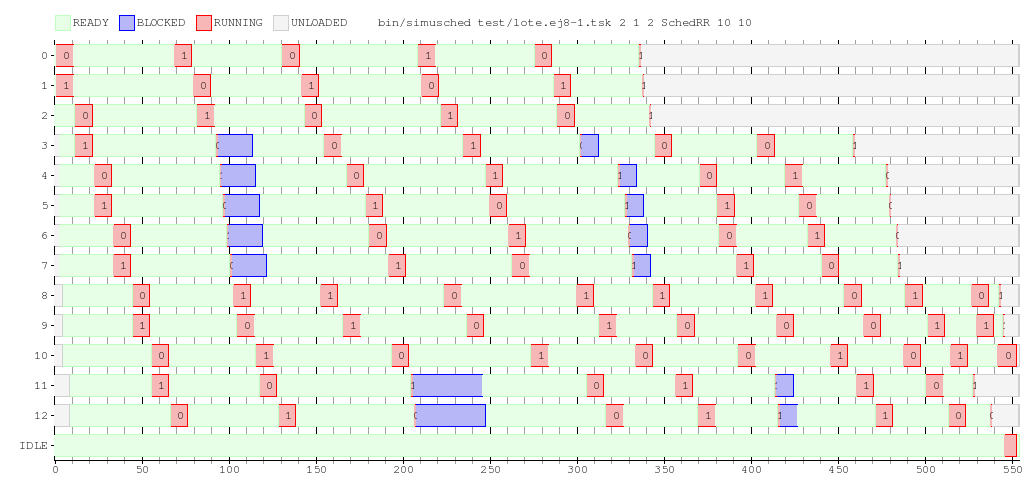
\includegraphics[scale=0.4]{imagenes/ej8-1-rr-c-2.png}
\end{center}
\caption{Round Robin con quantum 10, dos núcleos y costo de migración 2}
\end{figure}

\begin{figure}[H]
\begin{center}
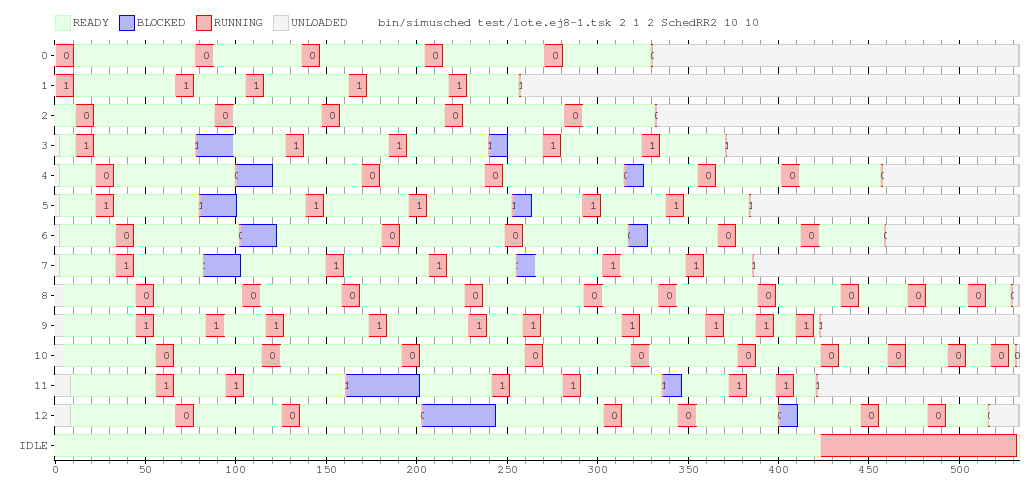
\includegraphics[scale=0.4]{imagenes/ej8-1-rr2-c-2.png}
\end{center}
\caption{Round Robin 2 con quantum 10, dos núcleos y costo de migración 2}
\end{figure}

\begin{figure}[H]
\begin{center}
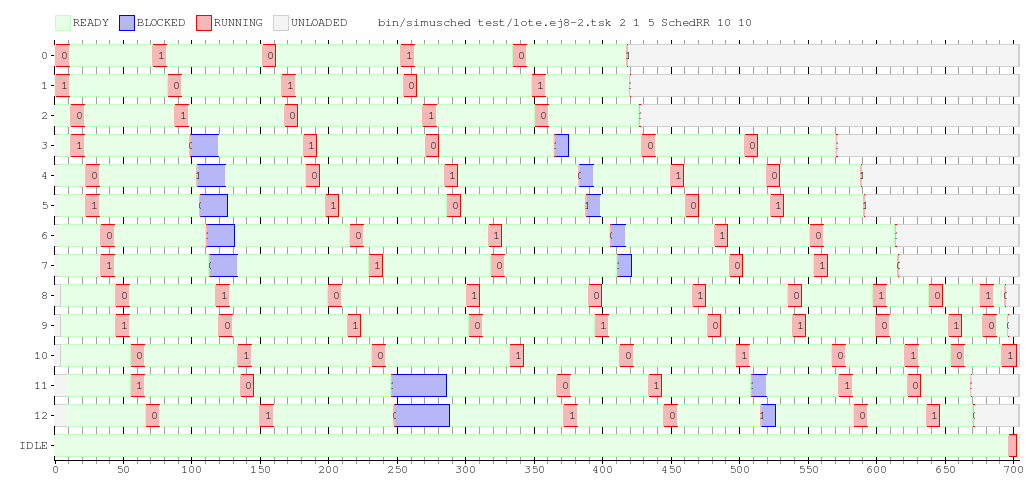
\includegraphics[scale=0.4]{imagenes/ej8-2-rr-c-2-m-5.png}
\end{center}
\caption{Round Robin con quantum 10, dos núcleos y costo de migración 5}
\end{figure}

\begin{figure}[H]
\begin{center}
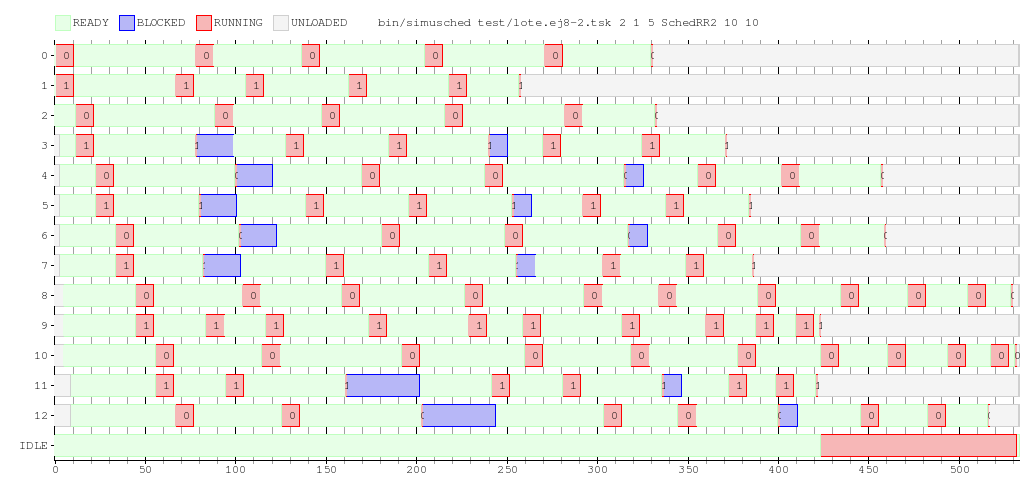
\includegraphics[scale=0.4]{imagenes/ej8-2-rr2-c-2-m-5.png}
\end{center}
\caption{Round Robin 2 con quantum 10, dos núcleos y costo de migración 5}
\end{figure}

\subsection{Conclusiones}

Como se puede observar en las gráficas 5 y 6, pese a que el \textit{Round
Robin 2} cuenta con menor \textit{turnaround}, presenta un mayor tiempo de
estado \textit{idle} en alguno de los núcleos. De esto se concluye que, pese
a que el tiempo total de ejecución disminuye con la nueva propuesta de
\textit{Round Robin 2}, se desperdician parte de los recursos que hay a
disposición, mientras que el enfoque clásico, pese a perder en performance,
hace un mejor uso de recursos.

Por las gráficas 7 y 8, podemos observar que al aumentar el costo de
migración de procesos entre núcleos, el algoritmo estándar de \textit{Round
Robin} es presenta un aumento aún mayor de \textit{turnaround}. De aquí se
concluye que el nuevo algoritmo propuesto es razonable para los casos en los
que la migración de procesos entre núcleos sea cara, como lo es en sistemas
embebidos, mientras que la primera implementación provee una flexibilidad
que, cuando dicho costo no es demasiado caro, puede ser beneficioso.

\section{Ejercicio 9}

\subsection{Metodología de experimentación}
Para este ejercicio se analizó el resultado de correr un lote determinado
(\verb|test/lote.ej9-1.tsk|) bajo el algoritmo de \textit{Lottery
scheduler} con 1000 semillas aleatorias distintas, pues no se podría
analizar ecuanimidad en una sola corrida, dada la naturaleza pseudoaleatoria
de este scheduler.

Para llevarlo a cabo, se analizó el uso de CPU de cada tarea durante los
primeros 40 ciclos de \textit{clock} en cada corrida, sin tener en cuenta el
tiempo gastado en cambio de contextos o el tiempo del núcleo en estado
\textit{idle}.

El objetivo de este experimento fue respaldar con evidencia empírica la
hipótesis de ecuanimidad del algoritmo de scheduling propuesta por los
autores.

\subsection{Resultados}
Al ser llevado a cabo el experimento, se obtuvo el siguiente resultado:

\begin{verbatim}
Tarea 0: 4822
Tarea 1: 4751
Tarea 2: 5101
Tarea 3: 4749
Tarea 4: 4853
Tarea 5: 4904
Tarea 6: 4816
Tarea 7: 5004
\end{verbatim}

Como se puede observar, el tiempo de CPU utilizado por cada proceso luego de
1000 corridas, oscila entre 4800 y 5200 ciclos de \textit{clock}, mientras
que el valor óptimo esperado es de 5000 ciclos. Esto demuestra que la
asignación de tiempo de CPU para cada proceso bajo el algoritmo de
\textit{Lottery scheduler} es ecuánime.

Si se desean repetir estos resultados, siguiendo las instrucciones del
apéndice, alcanza con ejecutar \verb|make plot; test/ej9-1.rb| en el
directorio principal.

\section{Ejercicio 10}

\subsection{Metodología}
Para llevar a cabo este experimento, se decidió ejecutar el \textit{Lottery
scheduler} 5 veces con la compensación implementada y sin ésta. Cada par de
corridas fue hecha con distintas semillas para números pseudoaleatorios con
el fin de generar distintos comportamientos del scheduler.

El obejetivo de este experimento es observar la falencia del scheduler sin
la implementación de compesaciones de \textit{tickets}, ya que sin ésta,
cuando una tarea no consume su total del quantum, está obteniendo menos
recursos del procesador que las demás, bajando la ecuanimidad.

El lote utilizado fue el siguiente:
\begin{verbatim}
TaskAlterno 1 15 1 15 1 15 1 15 1 15 1
@1
*3 TaskCPU 100
\end{verbatim}

\subsection{Resultados}

\begin{figure}[H]
\begin{center}
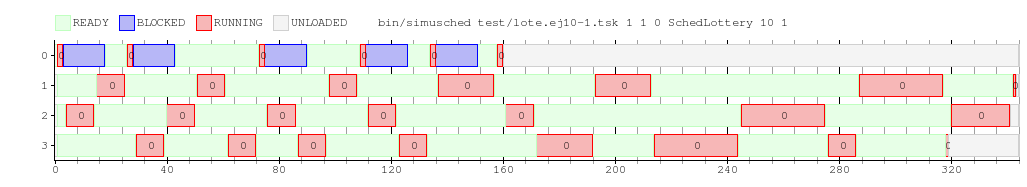
\includegraphics[scale=0.4]{imagenes/ej10-1-c-s-1.png}
\end{center}
\caption{con compensación, semilla = 1}
\end{figure}

\begin{figure}[H]
\begin{center}
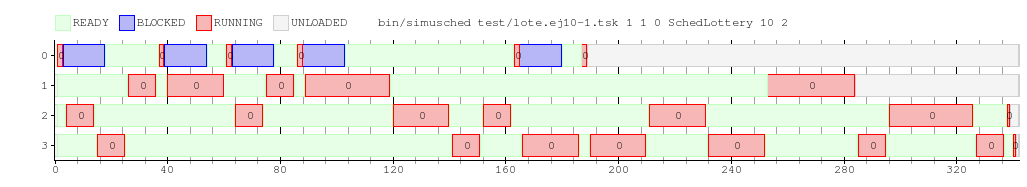
\includegraphics[scale=0.4]{imagenes/ej10-1-c-s-2.png}
\end{center}
\caption{con compensación, semilla = 2}
\end{figure}

\begin{figure}[H]
\begin{center}
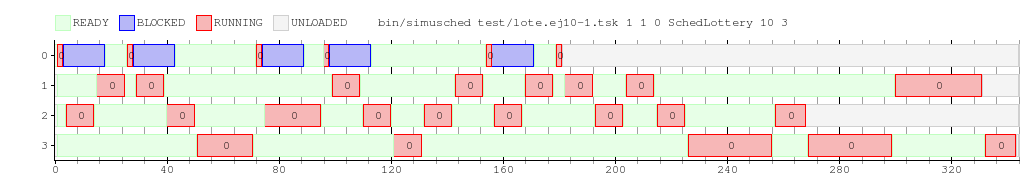
\includegraphics[scale=0.4]{imagenes/ej10-1-c-s-3.png}
\end{center}
\caption{con compensación, semilla = 3}
\end{figure}

\begin{figure}[H]
\begin{center}
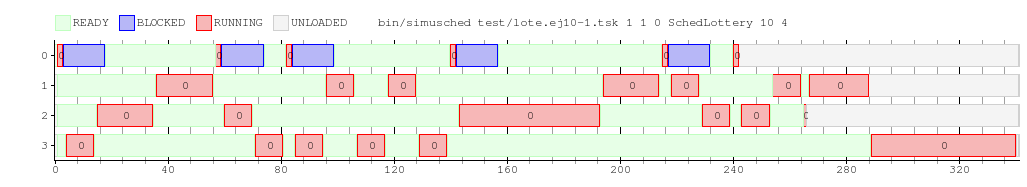
\includegraphics[scale=0.4]{imagenes/ej10-1-c-s-4.png}
\end{center}
\caption{con compensación, semilla = 4}
\end{figure}

\begin{figure}[H]
\begin{center}
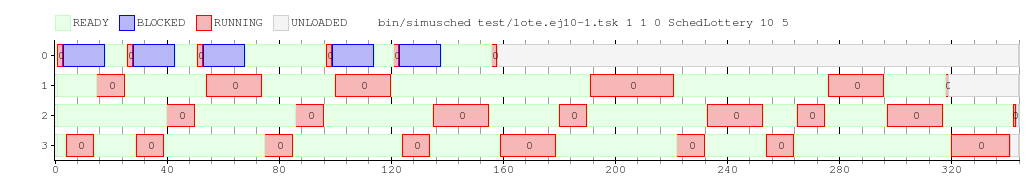
\includegraphics[scale=0.4]{imagenes/ej10-1-c-s-5.png}
\end{center}
\caption{con compensación, semilla = 5}
\end{figure}

\begin{figure}[H]
\begin{center}
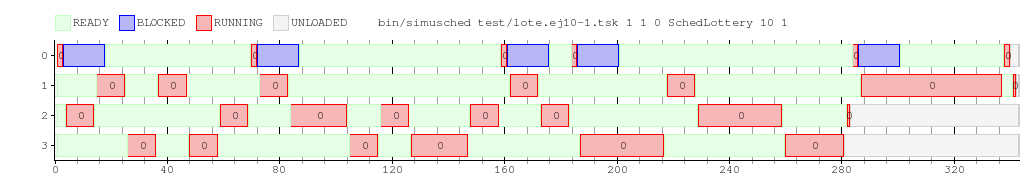
\includegraphics[scale=0.4]{imagenes/ej10-1-s-s-1.png}
\end{center}
\caption{sin compensación, semilla = 1}
\end{figure}

\begin{figure}[H]
\begin{center}
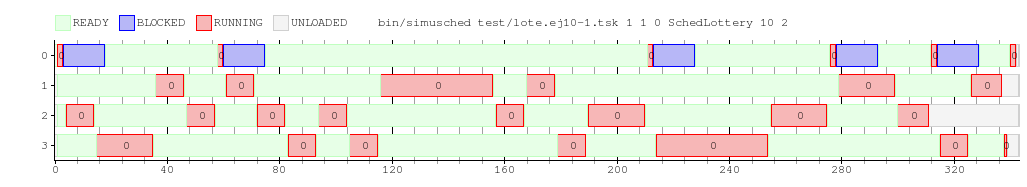
\includegraphics[scale=0.4]{imagenes/ej10-1-s-s-2.png}
\end{center}
\caption{sin compensación, semilla = 2}
\end{figure}

\begin{figure}[H]
\begin{center}
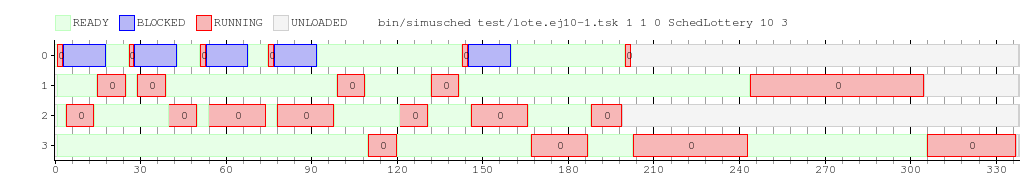
\includegraphics[scale=0.4]{imagenes/ej10-1-s-s-3.png}
\end{center}
\caption{sin compensación, semilla = 3}
\end{figure}

\begin{figure}[H]
\begin{center}
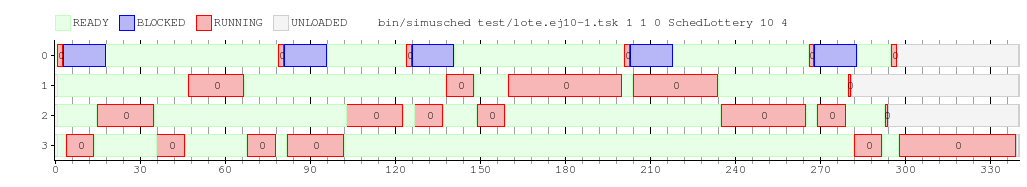
\includegraphics[scale=0.4]{imagenes/ej10-1-s-s-4.png}
\end{center}
\caption{sin compensación, semilla = 4}
\end{figure}

\begin{figure}[H]
\begin{center}
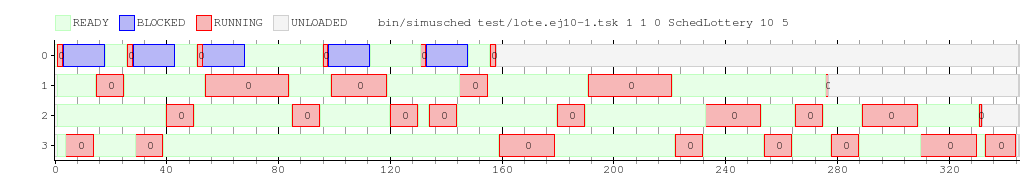
\includegraphics[scale=0.4]{imagenes/ej10-1-s-s-5.png}
\end{center}
\caption{sin compensación, semilla = 5}
\end{figure}

\section{Conclusión}

En las primeras 5 figuras (las correspondientes al scheduler con
compensación) se puede observar como la tarea que hace llamadas bloqueantes
gana la lotería de manera relativamente seguida debido a que su probabilidad
de salir elegida es mayor a la de las demás.

En las 5 imágenes posteriores se observa como la tarea $0$ espera intervalos
más grandes de tiempo que en las 5 primeras figuras, ésto es porque su
probabilidad de ganar es igual a las demás.

Este escenario denota la falencia de no tener una forma de compensación
sobre las tareas que no usan la totalidad de su cuota de procesador. Con lo
cual aquí se ve lo necesario de una forma de compensación para estas
situaciones, de otra forma la ecuanimidad se ve disminuida.

Una similitud que se notó en ambas implementaciones del scheduler fue que el
turnaround fue de 320 ciclos aproximadamente, es decir, el compensar o no
una tarea que no utiliza la totalidad de su tiempo no afecta el total de
ciclos consumiodos para terminar de ejecutar todos los procesos.

Observación: en el apéndice se adjuntan más imágenes de este experimento.

\section{Conclusion Final}

El trabajo hecho aquí nos pareció interesante. Hemos analizado  varios
schedulers y sus comportamientos con distintos tipos de tareas, y sus
ventajas y desventajas en dichas situaciones.


De hecho el lottery scheduler no es el único modelo de scheduling que sufre
este problema, las dos implementaciones de Round robin analizadas en este
trabajo, denotan la misma falencia.

\section{Apéndice}

Para compilar los archivos, basta situarse en el directorio \verb|tp1| y
ejecutar el \verb|make|. Para generar las imágenes del trabajo se debe
ejecutar en una terminal el comando \verb|make plot|. Para generar el
informe, se debe ejecutar \verb|make plot; make informe|.

Cabe destacar que es necesario tener instalado \verb|bash|, \verb|python|,
\verb|ruby|, \verb|make| y \verb|g++|.


\end{document}
